%!TEX program = xelatex
\documentclass[titlepage,11pt,a4paper]{article}
\usepackage{amssymb}
\usepackage{dsfont}
\usepackage{graphicx}
\usepackage[ruled,vlined]{algorithm2e}
\graphicspath{ {results/} }
\usepackage[titlepage]{polytechnique}


\title[INF 411 Programming Project]{Shortest Path Trees and Reach in Road Networks}
    %\subtitle{Le sous-titre (optionnel, enlever cette ligne sinon)}
    \author{Zuli \textsc{HUANG}\\
            Mingkun \textsc{LIU}
            }
    \date{09/01/2017}


\begin{document}
\maketitle

\section{Properties of Shortest-Path Trees}
To identify the number of different possible points we may be located in at the current moment of our trip, we choose the example vertex:
\begin{verbatim}
v 298251056 2277576 48783477
\end{verbatim}

\subsection{Question}{You have been traveling for time exactly t1 = 1 hour from the fixed starting point v towards your destination, which may be any sufficiently distant point in the network.}

We can obtain Figure \ref{fig:questioin_1.1_out} generated from the example vertex. Totally, there are 926 sufficiently distant points.
\begin{figure}[h]
    \centering
    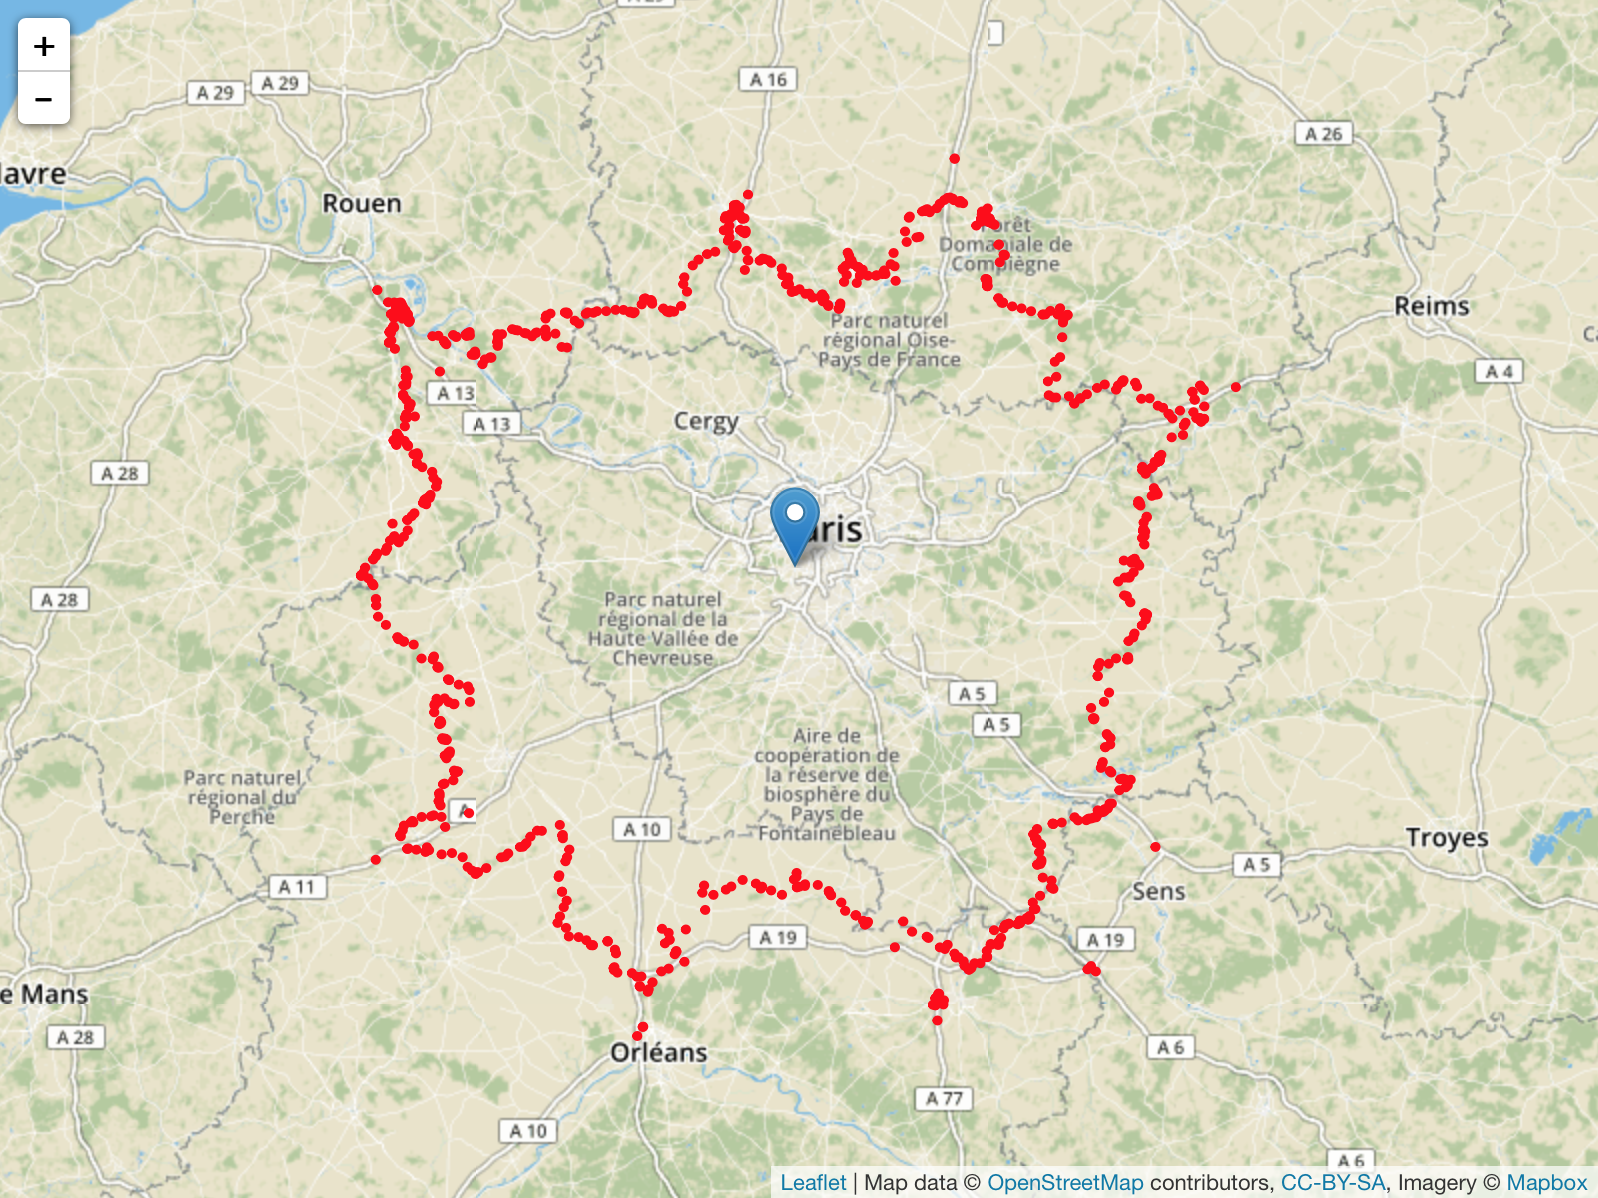
\includegraphics[width=\textwidth]{map_Q1.1.png}
    \caption{Points with 1h distance to vertex 298251056}
    \label{fig:questioin_1.1_out}
\end{figure}

\subsection{Question}{You have been traveling for time exactly t2 = 2 hours from the fixed starting point v towards your destination, which may be any sufficiently distant point in the network.}

It's similar to Q1.1. We choose the same center vertex v in the precedent question. And we obtain a map of sufficiently distant points. Totally, there are 2436 sufficiently distant ones.

\begin{figure}[h]
    \centering
    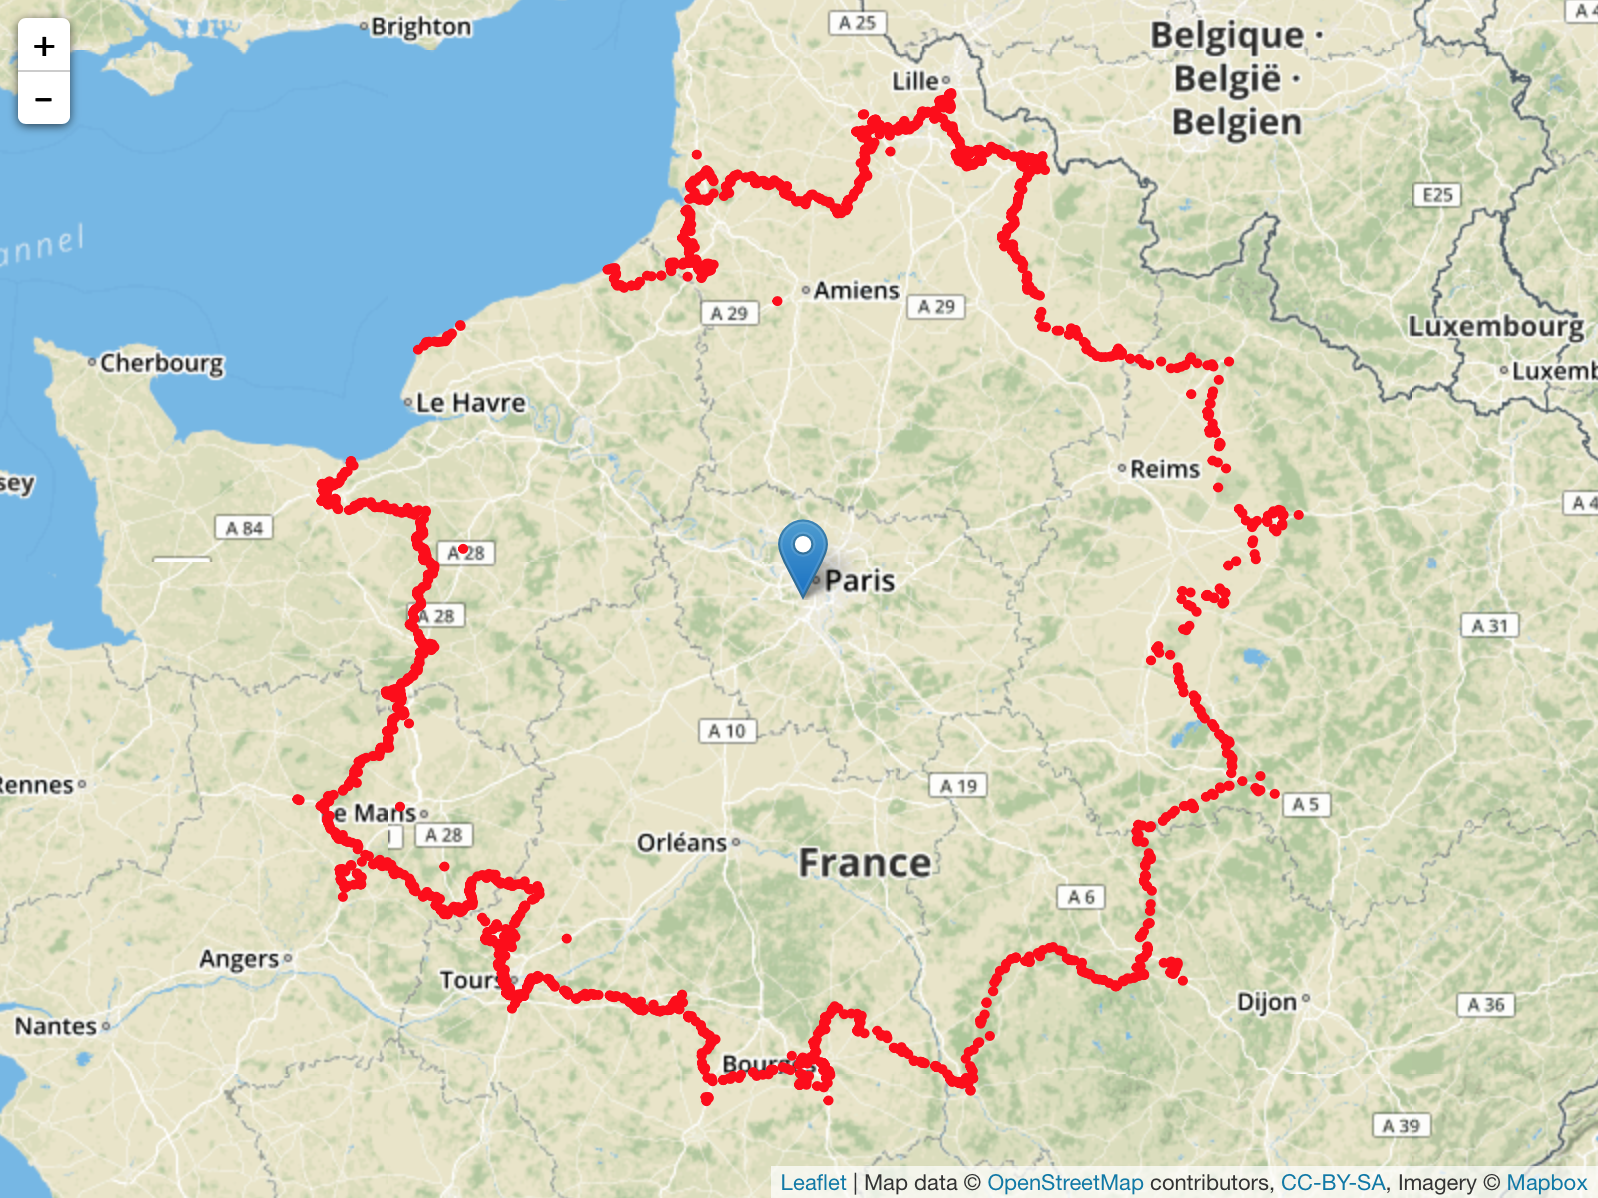
\includegraphics[width=\textwidth]{map_Q1.2.png}
    \caption{Points with 2h distance to vertex 298251056}
    \label{fig:questioin_1.2_out}
\end{figure}

\subsection{Question}{You have been traveling for time exactly t1 = 1 hour from the fixed starting point v towards your destination, when it is known that your destination is at least t2 = 2 hours' way away from your starting point v.}

We just need to back propagate points, obtained in the question 1.2, with 1h distance. And we get several appropriate points.

\newpage

\begin{figure}[h]
    \centering
    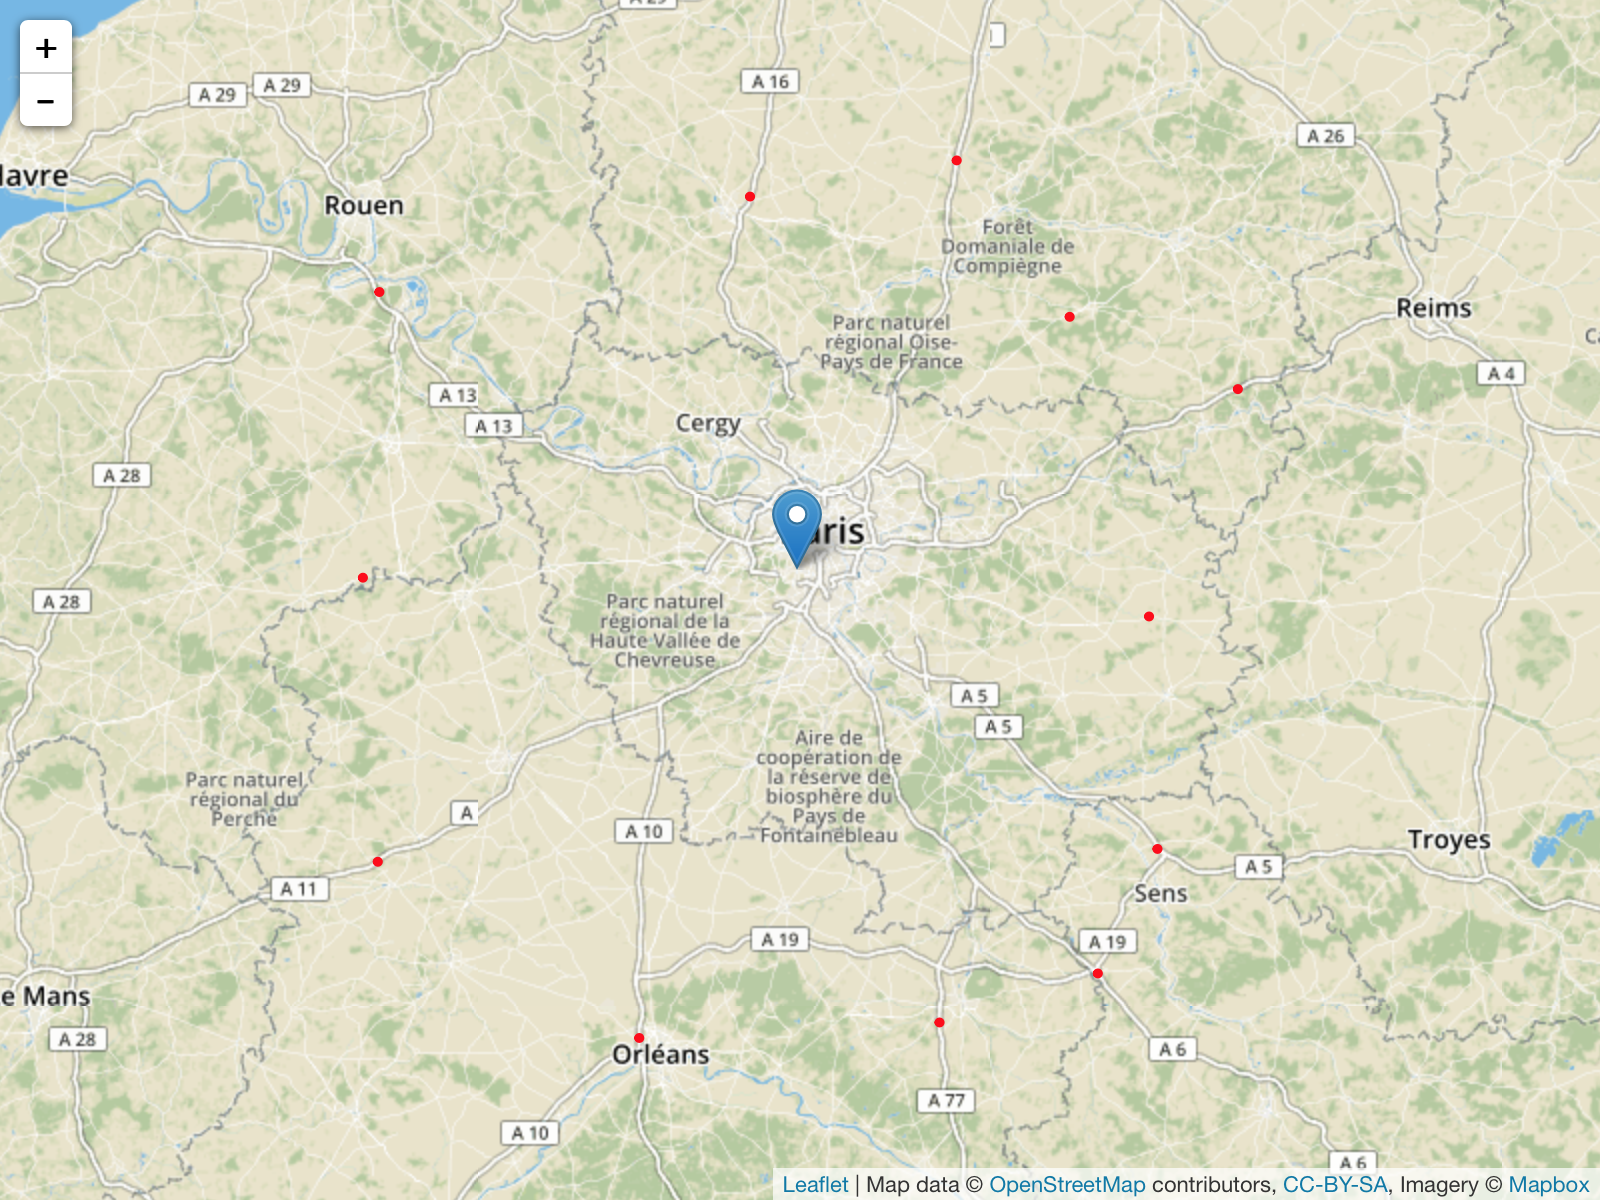
\includegraphics[width=\textwidth]{map_Q1.3.png}
    \caption{Points with 1h distance to v during a travel to a destination at least 2h away from v}
    \label{fig:questioin_1.3_out}
\end{figure}

\subsection{Methods}{Brief discussion of the graph algorithms used to answer the above questions.\\}
Algorithm that we use to handle question 1.1 to 1.3.

\begin{algorithm}[H]
 \KwData{An directed graph $G = (V, E)$, non negative wights, a source node $v\in V$, travel time $t$, $\omega : E \rightarrow \mathbb{R}$, $d : V \rightarrow \mathbb{R}$ distance to v, $settled : V \rightarrow boolean$}
 \KwResult{Set of points with distance $t$ to $v$}

 \For{$x \in V$}{
  settled(x) := false\;
  d(x) := $\infty$\;
 }
 Q.initialize, Qb.initialize\;

 \While{not Q.empty}{
  (x, prev, dist) := extractmin(Q, Qb)\;
  \eIf{$dist \leqslant d$}{
    \If{$dist > t $ and $d[prev] \leqslant t$}{
      points.add(x, prev, t-d[prev])\;
    }
   }
   {
   continue\;
   }

  \eIf {settled(x)} {
    continue\;
  }
  {settled(x) := true}

  \For{$y \in N(x)$}{
    \If{not settled(y)}{

      \If{$\omega(x, y) + d[x] \leqslant d[y]$}{
      d[y]:=$\omega(x, y) + d[x]$

      \eIf {$d[x] \leqslant t$}{
          Q.add(y, x, $\omega(x, y) + d[x]$);
        }
        {
          Qb.add(y, x, $\omega(x, y) + d[x]$);
        }

      p[y]:=x

      }
    }
  }

 }
 return points\;
 \caption{Find points with a certain distance to a given vertex}
\end{algorithm}
To find all sufficiently distant points without searching whole map, the main idea is to create two priority queues -- Q and Qb. Q stores the vertices whose predecessor can be visited within the travel time limit. Qb stores the vertices whose predecessor can't be visited within the travel time limit. It means that there is no more possible points when Q is empty. Another point is add a tuple element to priority queue, (vertex id, its predecessor id, distance). This point aims to successfully find those points, in different edge, that lead to the same vertex.
We can observe that there are few points obtained in Figure \ref{fig:questioin_1.3_out}. We can deduce that lots of vertices and edges will never be visited when we travel a sufficiently distant destination. And we find that the points in Figure \ref{fig:questioin_1.3_out} are all in "highways" connecting different cities.
\end{document}
